 
 
 \begin{figure}
 	\centering
 	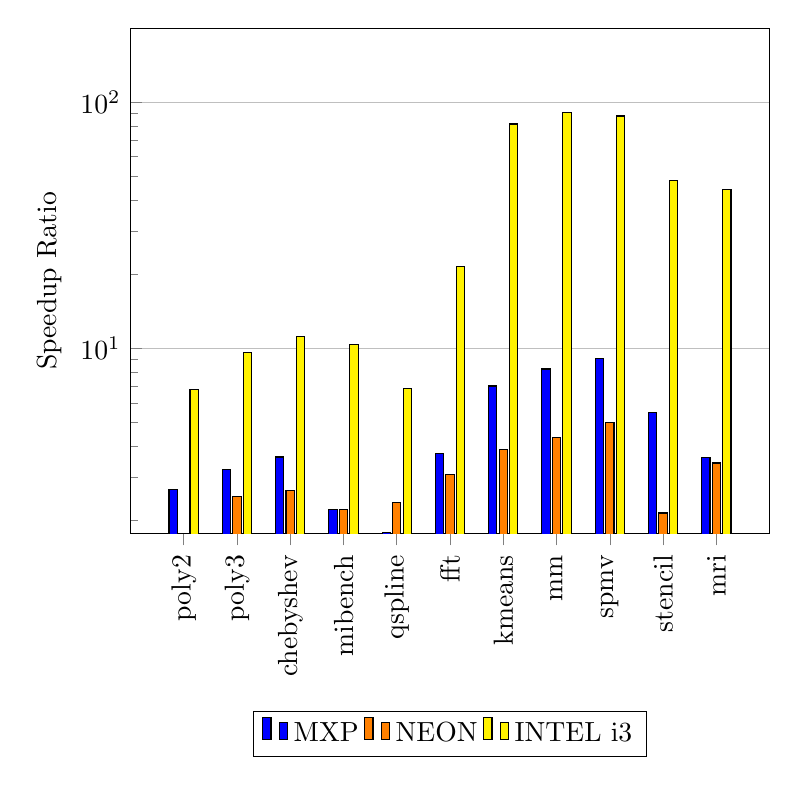
\begin{tikzpicture}
 	\begin{semilogyaxis}[
 	width  = 0.8*\textwidth,
 	height = 8cm,
 	xtick pos=left,
 	ytick pos=left,
 	%	major x tick style = transparent,
 	x tick label style={rotate=90, anchor=east, align=right,text width=2cm},
 	bar width=3pt,
 	ymajorgrids = true,
 	ylabel = {Speedup Ratio},
 	symbolic x coords={poly2,poly3,chebyshev,mibench,qspline,fft,kmeans,mm,spmv,stencil,mri},
 	xtick = data,
% 	nodes near coords,
% 	ybar,
% 	every node near coord/.append style={rotate=90, anchor=west,font=\tiny},
 	scaled y ticks = false,
 	enlarge y limits={upper,value=0.2},
 	%test
 	%	enlarge x limits=0.25,
 	ybar=2*\pgflinewidth,
 	legend cell align=left,
 	legend style={
 		at={(.5,-0.35)},
 		anchor=north,
 		legend columns=-1
 		column sep=0.5ex
 	}
 	]
 	\addplot[draw=black,fill=blue]
 	coordinates {(poly2,2.683) (poly3,3.21) (chebyshev,3.62) (mibench,2.216) (qspline,1.784) (fft,3.729) (kmeans,7.033) (mm,8.25) (spmv,9.11) (stencil,5.51) (mri,3.61) };
 	
 	\addplot[draw=black,fill=orange]
 	coordinates	{(poly2,1.769 ) (poly3,2.51) (chebyshev,2.638) (mibench,2.224) (qspline,2.3711) (fft,3.0811) (kmeans,3.90) (mm,4.335) (spmv,4.980) (stencil,2.146) (mri,3.424) };
 	
 	\addplot[draw=black,fill=yellow]
 	coordinates	{(poly2,6.78 ) (poly3,9.634) (chebyshev,11.18) (mibench,10.38) (qspline,6.855) (fft,21.45) (kmeans,81.5) (mm,90.8) (spmv,87.81) (stencil,48.12) (mri,44) };
 	
 	\legend{MXP,NEON,INTEL i3}
 	\end{semilogyaxis}	
 	\end{tikzpicture}
 	\caption{Half Word level Speedup Analysis w.r.t ARMv7 for  different benchmarks.}
 	\label{speedup:2}
 \end{figure}
 
